\section{Zmiana profilu}

Zmiana profilu to funkcjonalność umożliwiająca użytkownikom edycję podstawowych informacje na swój temat. Ma ona szczególne znaczenie i jest bardziej rozbudowana w przypadku wykonawców. Powodem jest to, że ustalane informacje są widoczne dla klientów i w ten sposób mogą wpłynąć na podejmowane przez nich wybory.

\begin{figure}[ht]
  \centering
  \begin{subfigure}[t]{0.33\textwidth}
    \centering
    \fbox{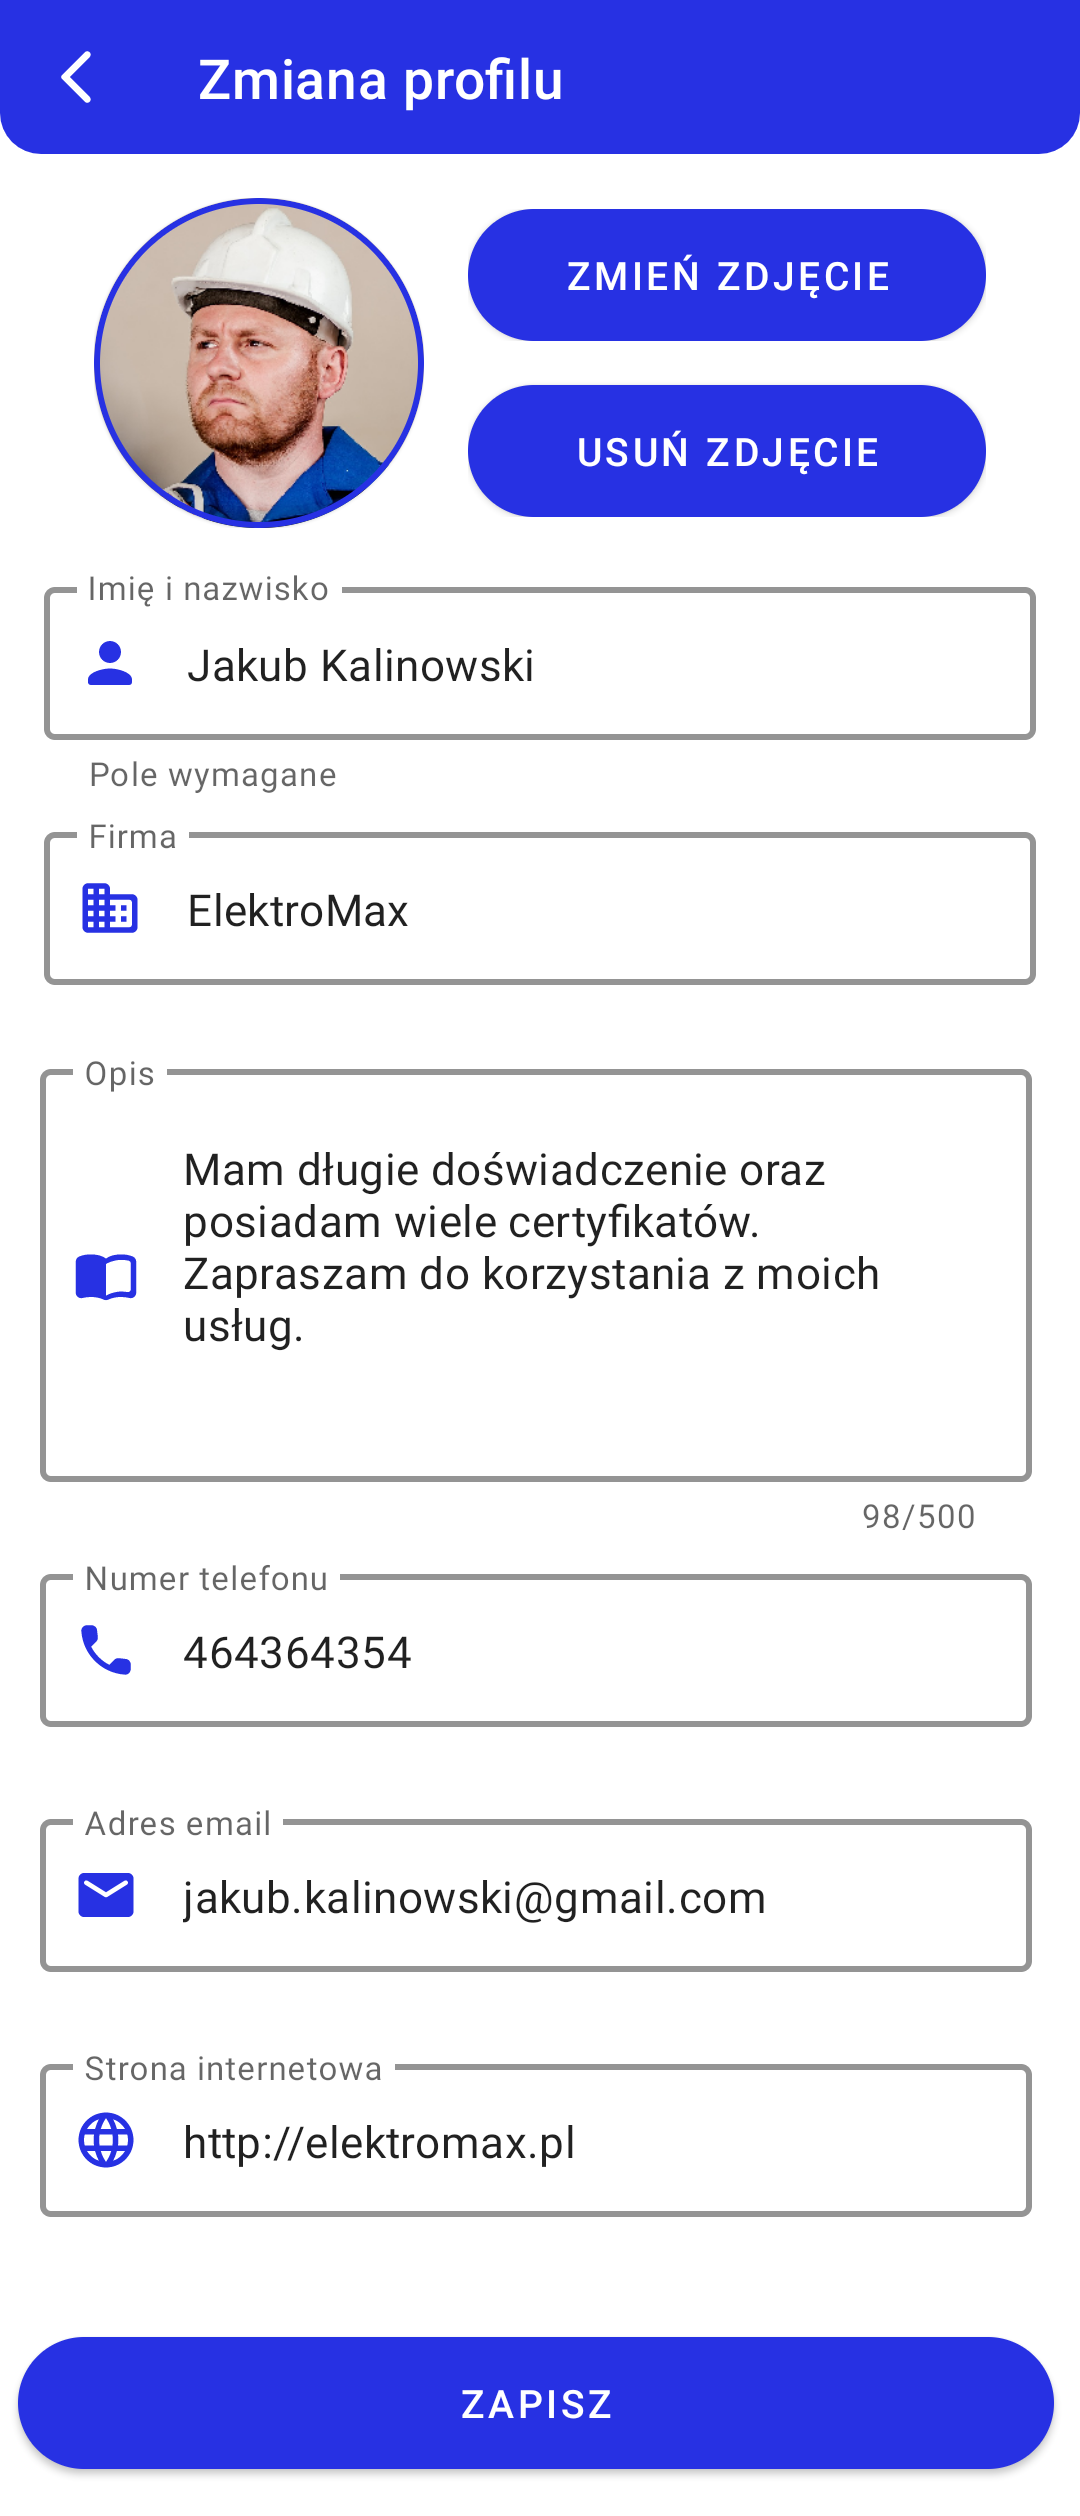
\includegraphics[width=0.97\linewidth]{screens/info_expert.png}}
    \caption{Widok wykonawców}
  \end{subfigure}
  \begin{subfigure}[t]{0.33\textwidth}
    \centering
    \fbox{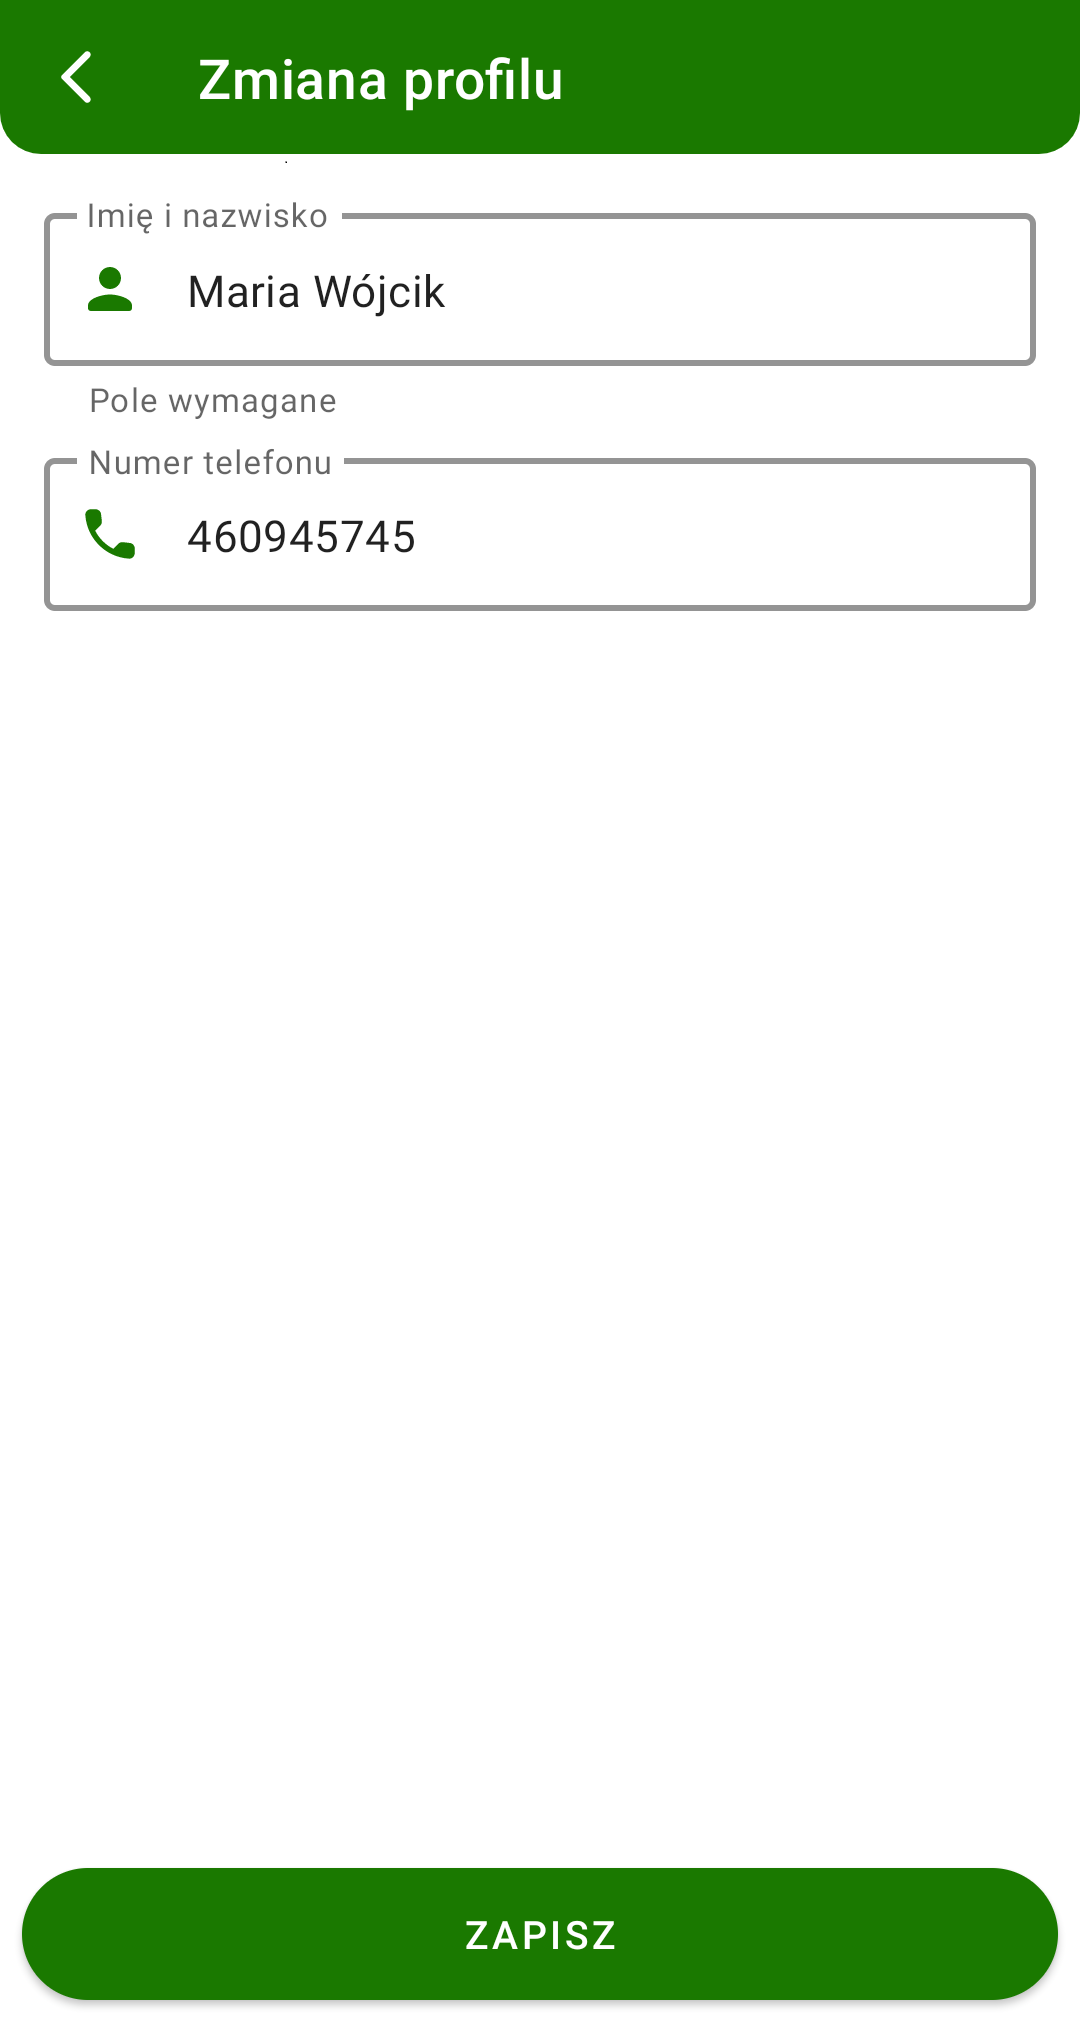
\includegraphics[width=0.97\linewidth]{screens/info_client.png}}
    \caption{Widok klientów}
  \end{subfigure}
  \caption{Ekran zmiany profilu}
  \label{fig:info-expert}
\end{figure}

Na rysunku \ref{fig:info-expert} przedstawione zostały ekrany zmiany profilu dla obu aplikacji. Jedynym elementem obligatoryjnym, który musi być na nich wypełniony, jest imię i nazwisko. Bez tego przycisk zapisu nie stanie się aktywny. Pozostałe pola są opcjonalne, lecz jeżeli zostaną wypełnione, a znajdujące się w nich dane nie będą poprawne, to przycisku zapisu również nie będzie można użyć. Wszystkie wartości są walidowane, a ewentualne informacje o błędach wyświetlane obok. Zostały wykorzystane w tym celu proste warunki, jak i wyrażenia regularne. Aplikacja dla wykonawców wyróżnia się obecnością komponentu do modyfikacji zdjęcia profilowego. Po wyrażeniu chęci jego zmiany na inne ukazuje się ekran służący do wyboru obrazu, a następnie przycięcia w kształt koła.

W kontekście zdjęć profilowych wykorzystany został interesujący mechanizm, aby zmniejszyć częstość ich pobierania. Jest to niepożądane z uwagi na generowany ruch sieciowy oraz koszty. Zdjęcia są oczywiście cachowane przez aplikacje klienckie, lecz jeśli byłyby wciąż wyciągane z pamięci podręcznej, to ich aktualizacje nie byłyby zauważane. Z tego powodu w bazie danych przechowywane są daty ostatnich ich modyfikacji. Dzięki temu możliwe jest ponowne pobranie zdjęcia profilowego jedynie wtedy, gdy zostanie zauważone, że ostatnia data jego modyfikacji została zmieniona na nowszą. Ogranicza to częstość pobierania zdjęć profilowych do minimum.

% Informacje widoczne na ekranach pobierane są bezpośrednio z bazy Firebase Firestore. Zapis wartości z pól tekstowych dokonywany jest natomiast poprzez jawnie wywoływaną funkcję Firebase Functions. Umożliwia ona przeprowadzenie walidacji danych w bezpiecznym środowisku przed ich utrwaleniem. Dodawanie, zmienianie oraz usuwanie zdjęć profilowych dokonuje się natomiast poprzez wykonywanie odpowiednich operacji na magazynie plików Firebase Storage.